\documentclass[11pt, oneside]{article} 
\usepackage{geometry}
\geometry{letterpaper} 
\usepackage{graphicx}
	
\usepackage{amssymb}
\usepackage{amsmath}
\usepackage{parskip}
\usepackage{color}
\usepackage{hyperref}

\graphicspath{{/Users/telliott_admin/Tex/png/}}
% \begin{center} 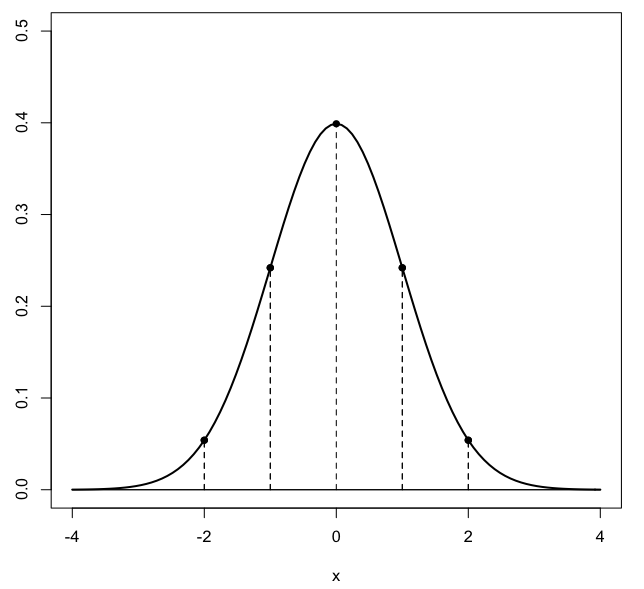
\includegraphics [scale=0.4] {gauss3.png} \end{center}

\title{Ceva's theorem}
\date{}

\begin{document}
\maketitle
\Large

\label{sec:Ceva}

Ceva's Theorem says that if we start with a triangle and draw line segments connecting each vertex with the midpoint of the opposite side, then the three line segments cross at a single, unique point.  The question is:  how do we know this?  We can obviously draw a line to the midpoint of the opposing side from two vertices, and these will cross at some point.
\begin{center} 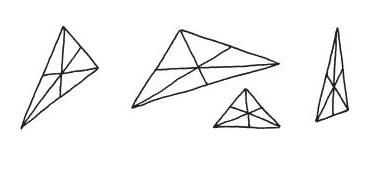
\includegraphics [scale=0.6] {Lockhart_Ceva.png} \end{center}

Then, we can either draw to the midpoint of the opposing side from the third vertex, and ask whether that line goes through the central point, or we can draw a line to the point and extend it to the opposing side, and then ask whether it bisects the side.  That's the question.  We will show that the answer is yes.

Furthermore, it is possible to show that for any of these line segments, this point (called the \emph{centroid}) lies one-third of the length from the side, and two-thirds of the length from the vertex.  We will use calculus to compute the centroid later in the book (and get the same answer).

In other write-ups I've shown one proof of this using similar triangles.  The first approach shown here is one outlined in Lockhart's book \emph{Measurement}.  And the second one uses vectors.

\subsection*{Lockhart's proof}
\begin{center} 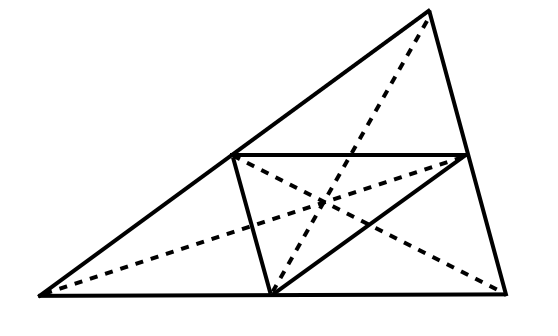
\includegraphics [scale=0.4] {ceva_small2.png} \end{center}

The idea is to connect the midpoints of the sides.  If we do that, the construction results in four smaller triangles.  It is easy to show that these triangles are congruent, and are similar to the large one we started with.  (By similar triangles, a short side opposite a midpoint/vertex is parallel to the side containing the midpoint.  I'm sure you can finish the proof).

Because of the congruent triangles, we also have three congruent parallelograms, and these have rotational symmetry around the centroid.  Therefore the centroid is a single point.

If you don't like that argument, notice that the dotted lines play the same role for each of the small triangles, extending from a vertex to the midpoint of the opposite side.  

What this means is that \emph{if} the centroid is a single point, then centroids of the larger triangle and the small central triangle are the same point.  But we can just continue in the same way, inscribing a new, even smaller, triangle, using the midpoints of the small central triangle, and this process can be extended \emph{ad infinitum}.  Hence, in the limit, we will reach a single point.

We can locate the centroid by imagining that we find successive midpoints of a length from opposite ends left and right.  The first point is at $1/2$ of the length (from the left), the second comes back from $1$ by $1/4$ so is at $0.75$ (at the right), the third is at $0.5 + 1/8$ (from the left), so every second round we get closer to the centroid  by advancing from the left by
\[ S = \frac{1}{2} +  \frac{1}{8} +  \frac{1}{32}  + \dots \]

Now, we can either assume this sum is finite (for now) or recognize that it is certainly smaller than 
\[ \frac{1}{2} +  \frac{1}{4} +  \frac{1}{8}  + \dots = 1 \]

\begin{center}
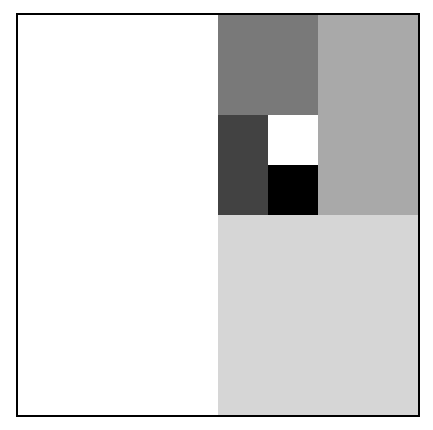
\includegraphics [scale=0.4] {series1.png}
\end{center}

So if
\[ S = \frac{1}{2} +  \frac{1}{8} +  \frac{1}{32}  + \dots \]
then
\[ 2S = 1 +  \frac{1}{4} +  \frac{1}{16}  + \dots \]
and
\[ 3S = 1S + 2S = 1 +  \frac{1}{2} +  \frac{1}{4} +  \frac{1}{8} + \frac{1}{16}   + \dots \]
That is, $3S = 1 + 1$, so $S = 2/3$.

\subsection*{using vectors}
Ceva's Theorem says that if we start with a triangle and draw the line segments connecting each vertex with the midpoint of the opposite side, the three line segments cross at a single, unique point.  Furthermore, it is possible to show that for any of these line segments, the \emph{centroid} lies one-third of the length from the side, and two-thirds of the length from the vertex.

Using vectors makes everything particularly simple.  As a warmup, let's start by looking at the midpoint of the diagonals for a parallelogram including the triangle of interest.  We will prove that the two diagonals cross at their mid-points (at $P$).
 \begin{center} 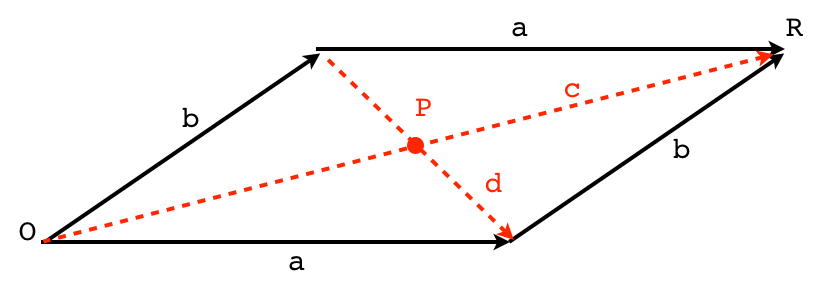
\includegraphics [scale=0.4] {ceva_vec1.png} \end{center}

by construction:
\[ \mathbf{c} = \mathbf{a} + \mathbf{b} \]
\[ \mathbf{b} + \mathbf{d} = \mathbf{a} \ \Rightarrow \  \mathbf{d} = \mathbf{a} - \mathbf{b}   \]

Let's define $P$ as the point we reach by going halfway along $\mathbf{c}$
\[  \mathbf{c} / 2 =  (\mathbf{a} + \mathbf{b})/2 \]

What we need to show is that if we do
\[ \mathbf{b} + \mathbf{d}/2 \]

we arrive at $P$.  Since $\mathbf{d} = \mathbf{a} - \mathbf{b}$
\[ \mathbf{b} + \mathbf{d}/2 = \mathbf{b} + (\mathbf{a} - \mathbf{b})/2 = (\mathbf{a} + \mathbf{b})/2 \]
$\square$

Vectors make that pretty easy.  We will use this result below.  Now, here is the triangle.
\begin{center} 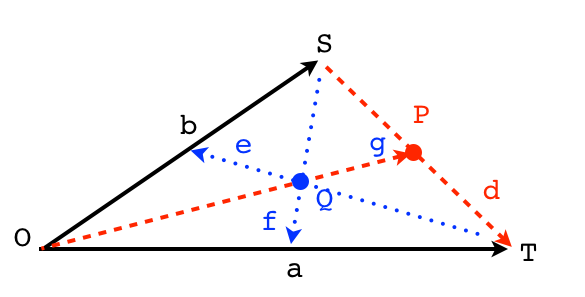
\includegraphics [scale=0.4] {ceva_vec2.png} \end{center}

Construct a line to the midpoint of the opposing side
\[ \mathbf{b} + \mathbf{f} =   \mathbf{a}/2 \ \Rightarrow \  \mathbf{f} =   \mathbf{a}/2 - \mathbf{b} \]
\[ \mathbf{a} + \mathbf{e} =  \mathbf{b}/2  \ \Rightarrow \  \mathbf{e} =   \mathbf{b}/2 - \mathbf{a} \]

Refer to the first diagram for $\mathbf{c} = (\mathbf{a} + \mathbf{b})$.  The halfway point is:
\[ \mathbf{a}/2 + \mathbf{b}/2 =  \mathbf{g}\]
By the property proved in the first part, we know that this bisects the side $\mathbf{d}$.

It makes it a little easier when we know that $Q$ is two-thirds of the way along the line segment.  We have three paths to move to $Q$.  The first two are constructed using the property that the vector bisects the opposing side.

from $S$:
\[ \mathbf{b} + \frac{2}{3} \mathbf{f} = \mathbf{b} +  \frac{2}{3}( \mathbf{a}/2 - \mathbf{b}) =  (\mathbf{a} + \mathbf{b})/3 \]
from $T$:
\[ \mathbf{a} + \frac{2}{3} \ \mathbf{e} = \mathbf{a} + \frac{2}{3} \ (\mathbf{b}/2 - \mathbf{a}) =  (\mathbf{a} + \mathbf{b})/3 \]
from $O$:
\[ \frac{2}{3} \mathbf{g} = \frac{2}{3} \ \frac{1}{2} \mathbf{c} = (\mathbf{a} + \mathbf{b})/3 \]
$\square$

By moving two-thirds of the way along $\mathbf{g}$, one-third of the way along $\mathbf{c}$, we arrive at the same point defined to be two-thirds of the way along the bisectors of opposing sides drawn from $S$ and $T$.

\subsection*{factor}
How would we find the factor of $2/3$ if we didn't already know?  Here is one way.  Call that unknown factor $r$.  By symmetry it is the same for all three lines.
\[ r \ (\mathbf{a} + \mathbf{b})/2 + (1-r) \ \mathbf{e} = \mathbf{b} / 2 \]
\[ r \ (\mathbf{a} + \mathbf{b})/2 + (1-r) \ (\mathbf{f} = \mathbf{a} / 2 \]
Substitute for $\mathbf{e}$ and $\mathbf{f}$:
\[ r \ (\mathbf{a} + \mathbf{b})/2 + (1-r) \ (\mathbf{b}/2 - \mathbf{a}) = \mathbf{b} / 2 \]
\[ r \ (\mathbf{a} + \mathbf{b})/2 + (1-r) \ (\mathbf{a}/2 - \mathbf{b}) = \mathbf{a} / 2 \]
add
\[ r \ (\mathbf{a} + \mathbf{b}) + (1-r) \ (-\mathbf{b}/2 - \mathbf{a}/2) = \mathbf{b} / 2 + \mathbf{b} / 2 \]
\[ \frac{3}{2} \ r \ (\mathbf{a} + \mathbf{b}) = \mathbf{a} + \mathbf{b} \]
\[ r = 2/3 \]

\end{document}